\chapter{Difração de Fraunhofer e filtragem espacial}\label{ch:b2:diffraction}

Aperte os olhos para um poste de luz através da fresta entre dois dedos e a
lâmpada se estica numa faixa de franjas; olhe uma estrela pelo
melhor dos telescópios e você verá não um ponto, mas um pequeno disco cercado
de círculos tênues. A luz que passa por uma abertura se espalha --- quanto
mais estreita a abertura, mais largo o espalhamento --- e nenhuma lente consegue
focalizá-la mais apertado do que esse espalhamento permite. É a
\emph{\omterm{def:b2:diffraction:huygens}{difração}}, a razão pela qual um microscópio não consegue ver um vírus, o
poder de resolução de um telescópio cresce com seu diâmetro e um feixe de
laser não consegue permanecer paralelo. Este capítulo calcula o padrão de
\omterm{def:b2:diffraction:huygens}{difração} de uma abertura no campo distante, o limite que ele impõe a todo
instrumento óptico, o modo como ele se combina com a interferência, e a
ideia --- de Abbe --- que faz do plano focal de uma lente um lugar onde uma
imagem pode ser filtrada.

\section{O princípio de Huygens--Fresnel e o regime de Fraunhofer}

\begin{definition}[Princípio de Huygens--Fresnel]\label{def:b2:diffraction:huygens}
\index{princípio de Huygens--Fresnel}\index{difração}\index{difração de Fraunhofer}
Todo ponto de uma \omterm{def:b2:scalar-light-model:path}{frente de onda} (ou de uma abertura iluminada por uma onda) age como
uma fonte secundária que emite uma ondícula esférica, em fase com a onda
ali; a onda além é a soma coerente das ondículas. Para uma
abertura $\Sigma$ iluminada por uma onda plana de amplitude $a$, a amplitude
que chega a um ponto distante é $\underline s(M) = K\iint_\Sigma\eu^{-\iu\varphi(P, M)}\dd S$, com
$\varphi(P, M)$ a fase do caminho do ponto $P$ da abertura até $M$
($K$ uma constante). A difração de \emph{Fraunhofer} (campo distante) é o caso
em que $M$ está no infinito --- ou no plano focal de uma lente --- de modo que
os raios que vão de todos os pontos da abertura até $M$ são paralelos, na
direção $\vect u$, e
\[
\varphi(P, M) = \varphi_0 - \frac{2\pi}\lambda\,\vect{OP}\cdot\vect u , \qquad
\underline s(\vect u) \propto \iint_\Sigma\eu^{\iu(2\pi/\lambda)\vect{OP}\cdot\vect u}\dd S .
\]
O padrão é observado no infinito, ou no foco $F'$ de uma lente,
onde a direção $\vect u$ de pequenos ângulos $(\alpha, \beta)$ corresponde ao
ponto $(f\alpha, f\beta)$.
\end{definition}
\admitted

\begin{remark}[Quando é longe o bastante?]\label{rem:b2:diffraction:fresnelnumber}
\index{número de Fresnel}
Para uma abertura de tamanho $D$ vista à distância $L$ sem lente, os
raios são suficientemente paralelos quando o termo quadrático do
\cref{exo:b2:scalar-light-model:12} é desprezível, $D^2/L \ll \lambda$ ---
o \emph{\omterm{rem:b2:diffraction:fresnelnumber}{número de Fresnel}} $D^2/\lambda L \ll 1$. Uma fenda de \qty{0.1}{mm} em
\qty{500}{nm} exige $L \gg \qty{2}{cm}$; uma abertura de \qty{1}{cm}, $L \gg \qty{200}{m}$ ---
daí a lente, que traz o infinito para seu plano focal. Mais perto
(\omterm{def:b2:diffraction:huygens}{difração} de Fresnel) os padrões são mais complexos; a sombra de uma
borda reta, por exemplo, tem franjas ao longo de seu lado iluminado.
\end{remark}

\section{A fenda única e a abertura circular}

\begin{proposition}[Difração por uma fenda]\label{prop:b2:diffraction:slit}
\index{difração por uma fenda}\index{função sinc}
Uma fenda de largura $b$ (longa ao longo de $y$) iluminada sob incidência normal envia na
direção $\theta$ (no plano perpendicular à fenda) a
intensidade
\[
I(\theta) = I_0\,\operatorname{sinc}^2\Bigl(\frac{\pi b\sin\theta}\lambda\Bigr) , \qquad \operatorname{sinc}x = \frac{\sin x}x :
\]
um máximo central brilhante de semilargura angular $\lambda/b$ (primeiros zeros em
$\sin\theta = \pm\lambda/b$), que contém $90\%$ da luz, e \omterm{thm:b2:gratings:nwaves}{máximos secundários}
em cerca de $\sin\theta = \pm1.43\lambda/b$, $\pm2.46\lambda/b$, \dots, de intensidades
relativas $4.7\%$, $1.6\%$, \dots --- quanto mais estreita a fenda, mais largo
o padrão. No plano focal de uma lente de distância focal $f$ o
máximo central tem $2\lambda f/b$ de largura.
\end{proposition}

\begin{proof}
$\underline s(\theta) \propto \int_{-b/2}^{b/2}\eu^{\iu kx\sin\theta}\dd x = b\,\operatorname{sinc}(kb\sin\theta/2)$
com $k = 2\pi/\lambda$; eleve ao quadrado. Zeros onde $b\sin\theta = m\lambda$, $m \ne 0$: as
ondículas das duas metades da fenda se cancelam então duas a duas.
\end{proof}

\begin{omfigure}
\begin{tikzpicture}[font=\small, x=1cm, y=1cm, >=Stealth]
  \begin{scope}
    \draw[thick] (0,-2) -- (0,-0.5) (0,0.5) -- (0,2);
    \draw[<->] (-0.35,-0.5) -- (-0.35,0.5) node[midway, left, font=\footnotesize] {$b$};
    \foreach \y in {-1.6,-0.9,-0.2,0.5,1.2} \draw[omDef, ->] (-2.2,\y) -- (-0.1,\y);
    \foreach \y in {-0.4,-0.2,0,0.2,0.4} \draw[omThm, thick, ->] (0.1,\y) -- (2.4,{\y+1.0});
    \draw[dashed] (0.1,0) -- (2.6,0); \draw (1.4,0) arc[start angle=0, end angle=23.5, radius=1.4]; \node[font=\footnotesize] at (1.7,0.28) {$\theta$};
    \node[font=\footnotesize] at (1.2,-1.6) {$b\sin\theta = \lambda$: primeiro zero};
  \end{scope}
  \begin{scope}[xshift=8.6cm]
    \begin{axis}[omaxis, axis x line=bottom, axis y line=left, width=6.4cm, height=4.4cm, at={(0,-2.0cm)},
        xlabel={$b\sin\theta/\lambda$}, ylabel={$I/I_0$}, xmin=-3.2, xmax=3.2, ymin=0, ymax=1.1, xtick={-3,-2,-1,0,1,2,3}, ytick={0.5,1}, samples=400,
        xlabel style={at={(axis description cs:0.5,-0.14)}, anchor=north},
        ylabel style={at={(axis description cs:-0.1,0.5)}, rotate=90, anchor=south}]
      \addplot[omDef, thick, domain=-3.2:3.2] {(sin(deg(pi*x))/(pi*x+1e-9))^2};
    \end{axis}
  \end{scope}
\end{tikzpicture}

{\small À esquerda: as ondículas vindas de toda a fenda, somadas na direção
$\theta$. À direita: o padrão de Fraunhofer da fenda, $\operatorname{sinc}^2$: um
lóbulo central duas vezes mais largo que os outros e muito mais brilhante.}
\end{omfigure}

\begin{proposition}[Abertura circular; o disco de Airy]\label{prop:b2:diffraction:airy}
\index{disco de Airy}\index{critério de Rayleigh (resolução)}\index{poder de resolução (instrumento)}
Uma abertura circular de diâmetro $D$ dá um disco central brilhante, o
\emph{\omterm{prop:b2:diffraction:airy}{disco de Airy}}, cercado de anéis tênues; o primeiro anel escuro está em
\[
\sin\theta = 1.22\,\frac\lambda D ,
\]
e o disco contém $84\%$ da luz. Todo instrumento com uma
pupila de entrada de diâmetro $D$ --- olho, câmera, telescópio, objetiva
de microscópio --- transforma uma fonte pontual num \omterm{prop:b2:diffraction:airy}{disco de Airy} desse raio
angular; dois pontos são \emph{resolvidos} (critério de Rayleigh) se sua
separação angular ultrapassa $1.22\lambda/D$: o poder de resolução do
instrumento.
\end{proposition}
\admitted

\begin{example}[O olho, o telescópio, o microscópio]\label{ex:b2:diffraction:instruments}
O olho ($D = \qty{3}{mm}$, $\lambda = \qty{550}{nm}$): $1.22\lambda/D = \qty{2.2e-4}{rad}$, cerca de
\qty{45}{''} --- um detalhe de \qty{1}{mm} a \qty{4}{m}, que é de fato mais ou menos a
acuidade de um bom olho: a evolução ajustou as células da retina ao
limite de \omterm{def:b2:diffraction:huygens}{difração}. Um telescópio de \qty{2.4}{m}: \qty{0.06}{''}, mil vezes
melhor, se a atmosfera deixar (do solo ela não deixa:
\qty{1}{''} de "seeing", daí os telescópios espaciais e a óptica adaptativa). Uma
antena de rádio de \qty{100}{m} em $\lambda = \qty{21}{cm}$: \qty{9}{'}, pior que o olho;
interferômetros entre continentes restauram a resolução. Uma
objetiva de microscópio de ângulo de abertura $\alpha$ resolve $0.61\lambda/n\sin\alpha$
--- cerca de \qty{0.2}{\micro m} no visível, seja qual for a ampliação: o
limite que levou a microscopia aos elétrons e aos raios X.
\end{example}

\begin{omfigure}
\begin{tikzpicture}[font=\small, x=1cm, y=1cm]
  \begin{scope}
    \foreach \r/\g in {1.5/85, 1.25/70, 1.0/50, 0.8/25, 0.6/5, 0.45/40, 0.3/70, 0.15/95} {
      \fill[black!\g] (0,0) circle (\r);
    }
    \node[font=\footnotesize] at (0,-1.9) {padrão de Airy de uma estrela};
  \end{scope}
  \begin{scope}[xshift=4.2cm]
    \foreach \r/\g in {0.8/25, 0.6/5, 0.45/40, 0.3/70, 0.15/95} {
      \fill[black!\g] (-0.45,0) circle (\r);
    }
    \foreach \r/\g in {0.8/25, 0.6/5, 0.45/40, 0.3/70, 0.15/95} {
      \fill[black!\g, opacity=0.6] (0.45,0) circle (\r);
    }
    \node[font=\footnotesize] at (0,-1.9) {duas estrelas no limite de Rayleigh};
  \end{scope}
  \begin{scope}[xshift=9.6cm]
    \begin{axis}[omaxis, axis x line=bottom, axis y line=left, width=5.4cm, height=4.0cm, at={(0,-1.8cm)},
        xlabel={$\theta D/\lambda$}, ylabel={$I$}, xmin=-2.5, xmax=3.5, ymin=0, ymax=1.5, xtick={-1.22,0,1.22,2.44}, xticklabels={$-1.22$,$0$,$1.22$,$2.44$}, ytick=\empty, samples=300,
        xlabel style={at={(axis description cs:0.5,-0.14)}, anchor=north},
        ylabel style={at={(axis description cs:-0.06,0.5)}, rotate=90, anchor=south}]
      \addplot[omDef, thick, domain=-2.5:3.5] {(sin(deg(pi*x/1.22))/(pi*x/1.22+1e-9))^2};
      \addplot[omThm, thick, domain=-2.5:3.5] {(sin(deg(pi*(x-1.22)/1.22))/(pi*(x-1.22)/1.22+1e-9))^2};
    \end{axis}
  \end{scope}
\end{tikzpicture}

{\small À esquerda e ao centro: o \omterm{prop:b2:diffraction:airy}{disco de Airy} de uma fonte pontual, e duas
fontes no limite de Rayleigh --- o centro de uma sobre o primeiro anel
escuro da outra. À direita: seus perfis (esboçados com formas em
$\operatorname{sinc}^2$), separados por $1.22\lambda/D$.}
\end{omfigure}

\section{Difração e interferência juntas}

\begin{proposition}[Fendas de Young de largura finita; a envoltória da rede]\label{prop:b2:diffraction:combined}
\index{envoltória (difração)}\index{ordens ausentes}
Duas fendas de largura $b$ cujos centros distam $a$ dão
\[
I(\theta) = 4I_0\,\operatorname{sinc}^2\Bigl(\frac{\pi b\sin\theta}\lambda\Bigr)\cos^2\Bigl(\frac{\pi a\sin\theta}\lambda\Bigr) :
\]
as franjas de Young (espaçamento $\lambda/a$ em $\sin\theta$) sob a envoltória
da fenda única (largura $2\lambda/b$); $a/b$ franjas preenchem o lóbulo central, e as
franjas em $a\sin\theta = p\lambda$ que caem sobre um zero da envoltória
($b\sin\theta = m\lambda$) estão \emph{ausentes}. Uma rede de $N$ fendas de largura
$b$ tem, do mesmo modo, seus \omterm{thm:b2:gratings:nwaves}{máximos principais} modulados pela mesma envoltória ---
que o blaze do \cref{ch:b2:gratings} inclina para a ordem em uso.
\end{proposition}

\begin{proof}
A integral sobre a abertura se separa numa soma, sobre as duas fendas, da mesma
integral deslocada de $\pm a/2$: $\underline s \propto b\,\operatorname{sinc}(\pi b\sin\theta/\lambda)
\times2\cos(\pi a\sin\theta/\lambda)$. Para $N$ fendas o segundo fator é a
soma de $N$ ondas.
\end{proof}

\begin{omfigure}
\begin{tikzpicture}
\begin{axis}[omaxis, axis x line=bottom, axis y line=left, width=13.6cm, height=4.6cm,
    xlabel={$a\sin\theta/\lambda$}, ylabel={$I/4I_0$}, xmin=-9, xmax=9, ymin=0, ymax=1.1, xtick={-8,-4,0,4,8}, ytick={0.5,1}, samples=1200,
    xlabel style={at={(axis description cs:0.5,-0.12)}, anchor=north},
    ylabel style={at={(axis description cs:-0.04,0.5)}, rotate=90, anchor=south}]
  \addplot[omDef, thick, domain=-9:9] {(sin(deg(pi*x/4))/(pi*x/4+1e-9))^2*cos(deg(pi*x))^2};
  \addplot[omThm, thick, dashed, domain=-9:9] {(sin(deg(pi*x/4))/(pi*x/4+1e-9))^2};
\end{axis}
\end{tikzpicture}

{\small Duas fendas com $a = 4b$: as franjas de Young sob a envoltória
da fenda única (tracejada); as franjas de quarta ordem caem sobre os zeros
da envoltória e estão ausentes.}
\end{omfigure}

\section{O plano de Fourier e a filtragem espacial}

\begin{proposition}[A lente como analisador de Fourier]\label{prop:b2:diffraction:fourier}
\index{plano de Fourier}\index{frequência espacial}\index{filtragem espacial}\index{teoria de Abbe}
Uma transparência de transmitância $t(x, y)$ no plano focal objeto de uma
lente, iluminada por uma onda plana, produz no plano focal imagem a
amplitude
\[
\underline s(X, Y) \propto \iint t(x, y)\,\eu^{-\iu2\pi(xX + yY)/\lambda f}\dd x\,\dd y
\]
--- sua transformada de Fourier bidimensional, com cada ponto $(X, Y)$ do
\emph{\omterm{prop:b2:diffraction:fourier}{plano de Fourier}} recolhendo a luz difratada nos ângulos
$(X/f, Y/f)$, ou seja, as \emph{\omterm{prop:b2:diffraction:fourier}{frequências espaciais}} $(X/\lambda f, Y/\lambda f)$ do
objeto: os detalhes finos (frequências altas) longe do eixo, os grosseiros
perto dele. Uma segunda lente reconstrói a imagem a partir desse plano; tudo o que
for bloqueado ou alterado ali fica filtrado fora da imagem
(\emph{\omterm{prop:b2:diffraction:fourier}{filtragem espacial}}, a \omterm{prop:b2:diffraction:fourier}{teoria de Abbe} do microscópio): um furo de agulha
no eixo guarda só as frequências baixas (suavização, "limpeza" de um
feixe de laser); um anteparo no eixo remove o fundo uniforme e
guarda as bordas (campo escuro, estrioscopia); uma \omterm{prop:b2:plane-waves-polarization:plates}{lâmina de quarto de onda} no
eixo transforma objetos de fase, invisíveis de outro modo, em contraste de intensidade
(contraste de fase, Zernike).
\end{proposition}

\begin{proof}[Justificativa]
Na integral de Fraunhofer, $\vect{OP}\cdot\vect u = x\alpha + y\beta$ com a
direção levada em $(X, Y) = (f\alpha, f\beta)$; a transmitância pondera
cada fonte secundária. (A própria transformada de Fourier é estudada no
volume de matemática do terceiro ano; aqui ela é apenas o nome desta integral.)
Para um objeto periódico de período $d$ a transformada é o conjunto das ordens
da rede em $X = p\lambda f/d$: a imagem só pode mostrar o período se pelo menos
as ordens $\pm1$ passarem pela lente --- a condição de Abbe, que é de novo
o limite de resolução do microscópio.
\end{proof}

\begin{omfigure}
\begin{tikzpicture}[font=\small, x=1cm, y=1cm, >=Stealth]
  \draw[omDef, thick, ->] (-5.6,0.8) -- (-4.6,0.8); \draw[omDef, thick, ->] (-5.6,0) -- (-4.6,0); \draw[omDef, thick, ->] (-5.6,-0.8) -- (-4.6,-0.8);
  \draw[thick, fill=omExo!20] (-4.4,-1.4) rectangle (-4.3,1.4); \node[font=\footnotesize] at (-4.35,-1.75) {objeto $t(x, y)$};
  \draw[thick, fill=omExo!20] (-2.4,0) ellipse (0.2 and 1.5); \node[font=\footnotesize] at (-2.4,-1.85) {$L_1$};
  \draw[thick] (0,-1.4) -- (0,1.4); \fill[omThm] (0,0) circle (2pt); \fill[omThm] (0,0.7) circle (1.5pt); \fill[omThm] (0,-0.7) circle (1.5pt);
  \node[font=\footnotesize] at (0,-1.75) {plano de Fourier};
  \draw[thick, fill=omExo!20] (2.4,0) ellipse (0.2 and 1.5); \node[font=\footnotesize] at (2.4,-1.85) {$L_2$};
  \draw[thick, fill=omExo!20] (4.3,-1.4) rectangle (4.4,1.4); \node[font=\footnotesize] at (4.35,-1.75) {imagem};
  \draw[omThm] (-4.35,0.6) -- (-2.4,1.0) -- (0,0.7) -- (2.4,0.4) -- (4.35,-0.6);
  \draw[omThm] (-4.35,-0.6) -- (-2.4,-1.0) -- (0,-0.7) -- (2.4,-0.4) -- (4.35,0.6);
  \draw[omProp] (-4.35,0.6) -- (-2.4,0.6) -- (0,0) -- (2.4,-0.6) -- (4.35,-0.6);
  \draw[omProp] (-4.35,-0.6) -- (-2.4,-0.6) -- (0,0) -- (2.4,0.6) -- (4.35,0.6);
  \draw[<->] (-4.35,1.7) -- (-2.4,1.7) node[midway, above, font=\footnotesize] {$f$}; \draw[<->] (-2.4,1.7) -- (0,1.7) node[midway, above, font=\footnotesize] {$f$};
  \node[omThm, font=\footnotesize, anchor=west] at (0.15,0.95) {ordens de um objeto periódico};
\end{tikzpicture}

{\small A montagem $4f$: a primeira lente forma a transformada de Fourier
do objeto em seu plano focal (um objeto periódico dá ali
ordens discretas), a segunda reconstrói a imagem; uma máscara no
\omterm{prop:b2:diffraction:fourier}{plano de Fourier} filtra a imagem.}
\end{omfigure}

\begin{example}[Limpar um feixe, ver o invisível]\label{ex:b2:diffraction:filtering}
Um feixe de laser carrega poeira e ondulações: focalize-o através de um furo de agulha de
alguns micrômetros --- o tamanho do \omterm{prop:b2:diffraction:airy}{disco de Airy} central do feixe
gaussiano limpo --- e todo o resto, que fica fora, é bloqueado;
o feixe recolimado é liso: um \emph{filtro espacial}. Uma célula viva
é transparente; ela muda apenas a fase da luz. Bloquear
a mancha axial torna suas bordas brilhantes sobre fundo preto; a lâmina de Zernike
desloca a luz não difratada de um quarto de onda para que ela interfira
em intensidade com a luz difratada: o interior da célula aparece,
e a biologia ganhou seu microscópio (prêmio Nobel de 1953).
\end{example}

\begin{method}[Estimativas de difração]\label{met:b2:diffraction:method}
(1) Espalhamento angular $\sim\lambda/b$ para uma abertura de tamanho $b$ ($1.22\lambda/D$ para
um círculo); o tamanho do padrão à distância $L$ ou com distância focal $f$ é
$\lambda L/b$, $\lambda f/b$. (2) Verifique a condição de Fraunhofer $b^2/\lambda L \ll 1$ ou
use uma lente. (3) Combine: envoltória de \omterm{def:b2:diffraction:huygens}{difração} $\times$ franjas de
interferência. (4) Resolução: dois pontos exigem $\Delta\theta > 1.22\lambda/D$; um objeto
periódico exige que suas primeiras ordens entrem na pupila. (5) A imagem do
\omterm{prop:b2:diffraction:fourier}{plano de Fourier}: o que bloquear para remover qual detalhe.
\end{method}

\section{Exercícios}

\begin{exercise}[$\star$]\label{exo:b2:diffraction:1}
Uma fenda de \qty{0.10}{mm} iluminada por um laser He--Ne (\qty{633}{nm}); anteparo a
\qty{2.0}{m}. Largura do máximo central; posição dos dois primeiros
\omterm{thm:b2:gratings:nwaves}{máximos secundários}; \omterm{rem:b2:diffraction:fresnelnumber}{número de Fresnel} --- o anteparo está longe o bastante? A mesma
fenda com uma lente de $f = \qty{50}{cm}$.
\end{exercise}

\begin{exercise}[$\star$]\label{exo:b2:diffraction:2}
Poder de resolução (Rayleigh) do olho (\qty{3}{mm}, \qty{550}{nm}); de um
telescópio amador de \qty{10}{cm}; do espelho de \qty{2.4}{m} do Hubble; de uma antena de rádio de \qty{64}{m}
em \qty{6}{cm}; de uma objetiva fotográfica de \qty{50}{mm} a $f/8$ (pupila de \qty{6}{mm}):
tamanho do \omterm{prop:b2:diffraction:airy}{disco de Airy} sobre o sensor, comparado a um pixel de \qty{4}{\micro m}.
\end{exercise}

\begin{exercise}[$\star$]\label{exo:b2:diffraction:3}
Duas fendas de largura $b = \qty{0.05}{mm}$, com centros a $a = \qty{0.25}{mm}$ de distância, $\lambda =
\qty{500}{nm}$, lente $f = \qty{1}{m}$: espaçamento das franjas; largura da envoltória
central; número de franjas nela; que ordens estão ausentes?
\end{exercise}

\begin{exercise}[$\star$]\label{exo:b2:diffraction:4}
Um feixe de laser de \qty{2}{mm} de diâmetro em \qty{633}{nm} se propaga até a Lua
(\qty{3.8e8}{m}): ângulo de \omterm{def:b2:diffraction:huygens}{difração} $\sim1.22\lambda/D$, diâmetro da mancha;
com um telescópio de \qty{3.5}{m} como emissor; por que os ecos da telemetria lunar são tão
fracos (o retrorrefletor, de \qty{1}{m}, devolve a luz com sua própria
\omterm{def:b2:diffraction:huygens}{difração})?
\end{exercise}

\begin{exercise}[$\star\star$]\label{exo:b2:diffraction:5}
\emph{A fenda em detalhe.} (a) Efetue a integral de Fraunhofer para
a fenda e obtenha $\operatorname{sinc}^2$. (b) Mostre que os \omterm{thm:b2:gratings:nwaves}{máximos secundários}
estão em $\tan x = x$ ($x = \pi b\sin\theta/\lambda$), o primeiro perto de $x = 1.43\pi$, e
calcule sua intensidade relativa. (c) Fração da energia no
lóbulo central (admita $\int_{-\pi}^\pi\operatorname{sinc}^2 = 0.903\pi$ e
$\int_{-\infty}^\infty\operatorname{sinc}^2 = \pi$). (d) A fenda é iluminada sob incidência
$\theta_0$: mostre que o padrão é o mesmo, centrado na direção $\theta_0$.
\end{exercise}

\begin{exercise}[$\star\star$]\label{exo:b2:diffraction:6}
\emph{Microscópio.} Uma objetiva de \omterm{prop:b2:guided-waves:fibre}{abertura numérica} $n\sin\alpha = 1.4$
(imersão em óleo) em \qty{500}{nm}: menor distância resolvida $0.61\lambda/n\sin
\alpha$; com luz azul (\qty{400}{nm}); no ultravioleta (\qty{250}{nm}); por que
uma ocular de $1000\times$ não ajuda (o limite do próprio olho a \qty{25}{cm} é
\qty{0.1}{mm})? O que mudam os microscópios eletrônicos ($\lambda = \qty{4}{pm}$ a
\qty{100}{keV})?
\end{exercise}

\begin{exercise}[$\star\star$]\label{exo:b2:diffraction:7}
\emph{Retangular e circular.} (a) Para uma abertura retangular $b \times h$:
mostre que o padrão vale $\operatorname{sinc}^2(\pi b\sin\theta_x/\lambda)\operatorname{sinc}^2(\pi h
\sin\theta_y/\lambda)$: uma cruz, mais larga ao longo do lado mais estreito. (b) Um quadrado de
\qty{0.2}{mm} com $f = \qty{1}{m}$: tamanho do quadrado central. (c) Para um
círculo de mesma largura o primeiro zero está em $1.22\lambda/D$ em vez de $\lambda/b$:
por que mais longe (pense na luz concentrada perto do centro de um
disco)? (d) O espelho secundário de um telescópio é sustentado por quatro hastes: o que
elas acrescentam à imagem de uma estrela brilhante?
\end{exercise}

\begin{exercise}[$\star\star$]\label{exo:b2:diffraction:8}
\emph{Abbe.} Uma rede de período $d = \qty{2}{\micro m}$ é observada com uma
objetiva de microscópio de ângulo de abertura $\alpha$ no ar, $\lambda = \qty{550}{nm}$.
(a) Ângulos de suas ordens $\pm1$, $\pm2$. (b) $\sin\alpha$ mínimo para que a imagem
mostre o período (as ordens $\pm1$ devem entrar). (c) Com $\sin\alpha = 0.4$: o que
a imagem mostra --- é uma rede fiel? (d) A iluminação
oblíqua deixa passar a ordem zero e \emph{uma} primeira ordem:
$\sin\alpha$ mínimo então, e o ganho.
\end{exercise}

\begin{exercise}[$\star\star$]\label{exo:b2:diffraction:9}
\emph{Filtro espacial.} Um feixe de laser de \qty{2}{mm} ($\lambda = \qty{633}{nm}$) é
focalizado por uma lente de $f = \qty{20}{mm}$ através de um furo de agulha. (a) Diâmetro do
\omterm{prop:b2:diffraction:airy}{disco de Airy} central no foco; diâmetro do furo para deixá-lo passar
(tome $1.5\times$). (b) Um grão de poeira de \qty{50}{\micro m} sobre o feixe
difrata a luz em que ângulo, e onde essa luz cai no
plano focal --- passa pelo furo ou não? (c) Potência perdida se o feixe
for gaussiano e o furo deixar passar $99\%$ dele; por que o feixe emergente
é liso? (d) Por que o furo precisa estar centrado com precisão de alguns
micrômetros?
\end{exercise}

\begin{exercise}[$\star\star\star$]\label{exo:b2:diffraction:10}
\emph{Babinet.} Dois anteparos complementares (uma fenda e uma tira
opaca de mesma largura) são iluminados por uma onda plana. (a) Mostre que, fora
da direção do feixe incidente, seus padrões de Fraunhofer
são idênticos (a soma das duas amplitudes é a da
onda sem obstáculo, nula fora do eixo). (b) O padrão de um fio de cabelo de
diâmetro \qty{80}{\micro m} a \qty{2}{m} com um laser: espaçamento das franjas, e o
diâmetro do cabelo a partir dele --- uma medida clássica. (c) O que se vê
sobre o próprio eixo? (d) Por que gotículas pequenas numa nuvem fina produzem uma
coroa de anéis coloridos em torno da Lua, e o que dá o raio
dos anéis?
\end{exercise}

\begin{exercise}[$\star\star\star$]\label{exo:b2:diffraction:11}
\emph{Campo escuro e contraste de fase.} Um objeto transparente tem
$t(x) = \eu^{\iu\varphi(x)} \approx 1 + \iu\varphi(x)$ com $|\varphi| \ll 1$. (a) Intensidade de
sua imagem comum: mostre que ela é uniforme em primeira ordem --- invisível. (b)
No \omterm{prop:b2:diffraction:fourier}{plano de Fourier} o "1" é a mancha axial e $\iu\varphi$ a
luz difratada em torno dela: se um anteparo bloqueia a mancha axial, a intensidade
da imagem vale $\propto\varphi^2$ --- campo escuro; sua fraqueza. (c) Se, em vez disso, a
mancha axial é atrasada de $\pi/2$ (multiplicada por $\iu$): imagem $\propto|1 +
\varphi|^2 \approx 1 + 2\varphi$ --- contraste de fase, linear em $\varphi$. (d) Por que a
lâmina de Zernike é muitas vezes também absorvente (ela atenua a mancha axial)?
\end{exercise}

\begin{exercise}[$\star\star\star$]\label{exo:b2:diffraction:12}
\emph{Resolução da imagem da fenda de um espectrógrafo e a rede.} Uma
rede de largura $W$ é a abertura do espectrógrafo: mostre que o
padrão de \omterm{def:b2:diffraction:huygens}{difração} dessa abertura, $\operatorname{sinc}^2(\pi W\sin\theta/\lambda)$
(para o feixe que sai em $\theta \approx 0$), tem semilargura angular
$\lambda/W$, e que, convertida em comprimento de onda pela dispersão $p/a\cos
\theta$, isso dá $\Delta\lambda = \lambda/pN$ --- o poder de resolução do
\cref{ch:b2:gratings}, visto como \omterm{def:b2:diffraction:huygens}{difração}. (b) Um telescópio de
diâmetro $D$ e uma rede de largura $W$: a rede deve ser mais larga que
$D\,f_{\text{col}}/f_{\text{tel}}$: por quê? (c) Explique numa frase por que
todo "poder de resolução" em óptica é $\sim$(tamanho da abertura)/$\lambda$.
(d) O que a fenda acrescenta, e quando ela domina?
\end{exercise}

\begin{omfigure}
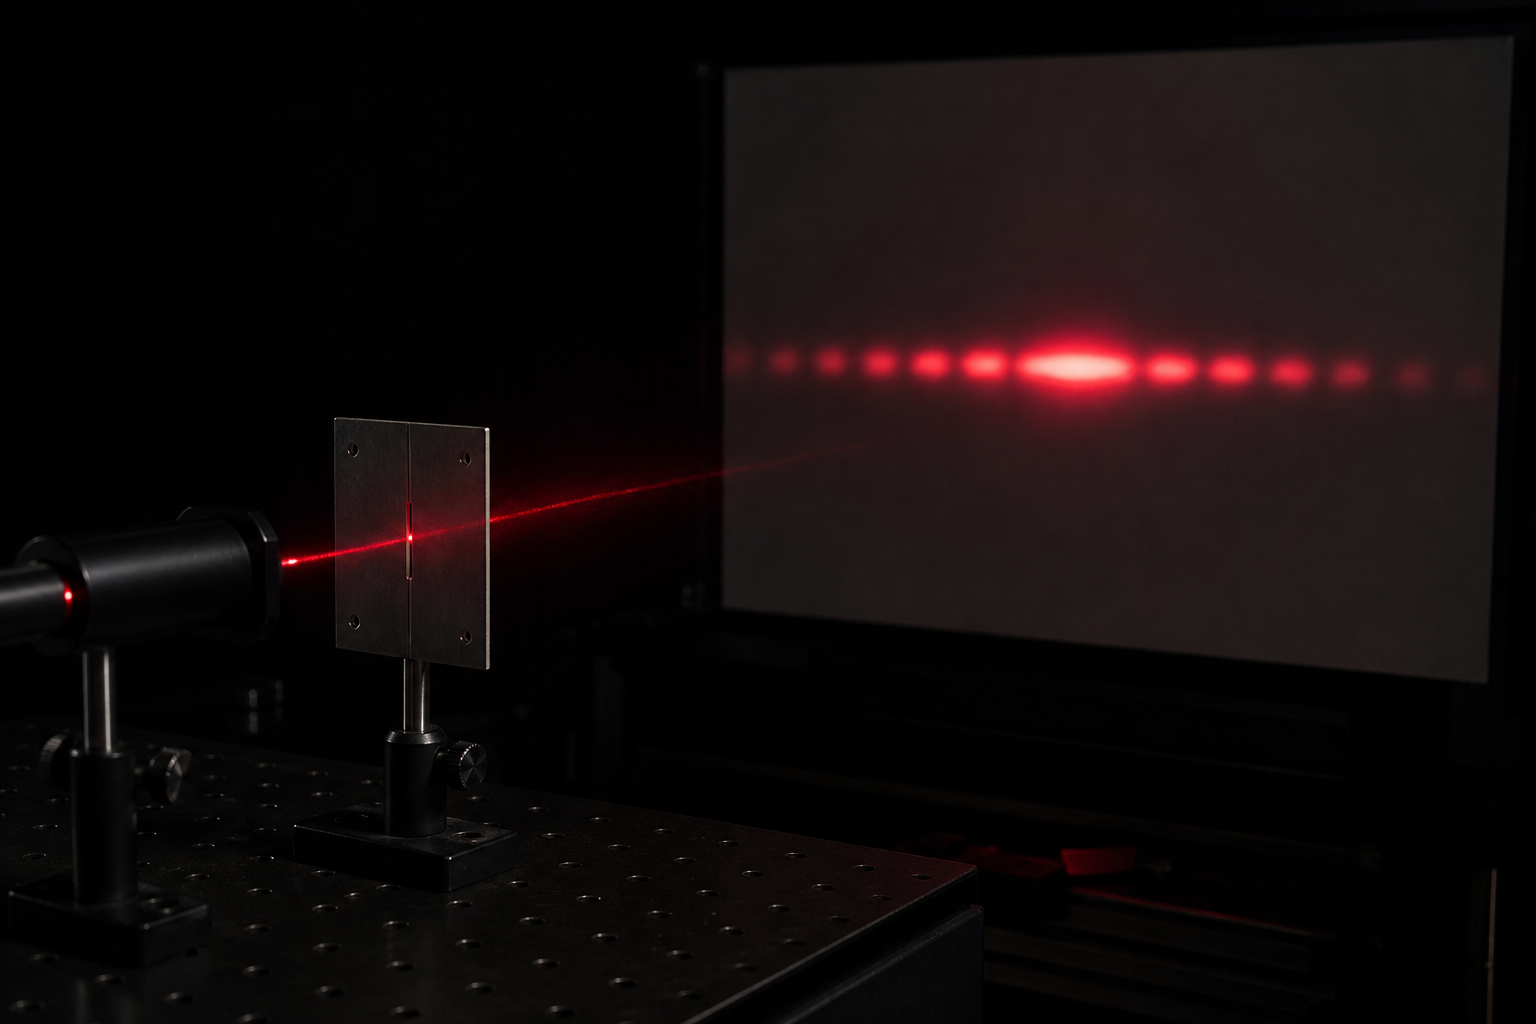
\includegraphics[width=0.58\linewidth]{images/book4/ai/b4-22-slit-diffraction-pattern.png}

{\small Um feixe de laser através de uma fenda estreita: no anteparo distante, a larga banda central brilhante e os máximos laterais mais fracos e mais estreitos do padrão de Fraunhofer.}
\end{omfigure}

\section{Problema: o que se pode resolver}

\begin{problem}[{Problema de fim de semana --- o limite de difração em quatro
escalas: o olho, um telescópio, um microscópio e o feixe de laser que
deve ser limpo antes de ser usado}]
\label{pb:b2:diffraction:1}

\medskip
\noindent\textbf{Parte I --- O olho.}
Pupila $D = \qty{3}{mm}$ de dia, \qty{7}{mm} à noite; $\lambda = \qty{550}{nm}$; os
cones da retina estão a \qty{2}{\micro m} um do outro na fóvea, e a distância
focal do olho é \qty{17}{mm}.
\begin{enumerate}
  \item Raio angular do \omterm{prop:b2:diffraction:airy}{disco de Airy} de dia; seu raio linear sobre
        a retina; compare com o espaçamento dos cones --- a retina está
        ajustada à óptica?
  \item Menor separação de dois pontos resolvida a \qty{25}{cm}; a
        \qty{10}{m}; você consegue ler um texto de \qty{1}{mm} com o braço estendido?
  \item À noite a pupila abre até \qty{7}{mm}: limite de \omterm{def:b2:diffraction:huygens}{difração} então;
        por que a visão ainda assim piora (aberrações do
        cristalino em plena abertura, bastonetes mais grosseiros que os cones)?
  \item Dois faróis de carro a \qty{1.5}{m} um do outro: distância a partir da qual eles se fundem
        numa só luz.
  \item Um furo de \qty{1}{mm} diante do olho: o que faz a \omterm{def:b2:diffraction:huygens}{difração},
        e por que um furo de agulha ainda assim ajuda um olho míope
        (profundidade de campo)?
\end{enumerate}

\medskip
\noindent\textbf{Parte II --- O telescópio.}
Um telescópio de \qty{1}{m}, $f = \qty{10}{m}$, com uma câmera de pixels de \qty{10}{\micro m};
$\lambda = \qty{550}{nm}$.
\begin{enumerate}[resume]
  \item Limite de \omterm{def:b2:diffraction:huygens}{difração} em segundos de arco; raio de Airy sobre o
        detector; pixels por \omterm{prop:b2:diffraction:airy}{disco de Airy}.
  \item A atmosfera borra as imagens até \qty{1}{''}: quanto se perde da
        resolução do telescópio? Diâmetro de telescópio para o qual
        o limite de \omterm{def:b2:diffraction:huygens}{difração} se iguala ao seeing.
  \item A óptica adaptativa corrige a atmosfera em \qty{2.2}{\micro m}:
        limite de \omterm{def:b2:diffraction:huygens}{difração} ali; por que é mais fácil no infravermelho?
  \item Uma estrela dupla com componentes a \qty{0.15}{''}: resolvida com
        óptica adaptativa em \qty{2.2}{\micro m}? E em \qty{550}{nm} a partir do espaço?
  \item A Lua está a \qty{3.8e5}{km}: menor cratera que este telescópio
        poderia resolver (só a \omterm{def:b2:diffraction:huygens}{difração}); e a pegada de um módulo
        lunar (\qty{4}{m})?
  \item Poder coletor de luz do telescópio em relação ao
        olho noturno (\qty{7}{mm}); o que isso traz, e o que não traz.
  \item A luz de uma estrela através das quatro hastes que sustentam o
        espelho secundário: descreva a imagem.
\end{enumerate}

\medskip
\noindent\textbf{Parte III --- O microscópio.}
Objetiva de \omterm{prop:b2:guided-waves:fibre}{abertura numérica} $\mathrm{NA} = n\sin\alpha = 0.9$ (a seco) ou $1.4$
(em óleo), $\lambda = \qty{550}{nm}$; a distância resolvida vale $0.61\lambda/\mathrm{NA}$.
\begin{enumerate}[resume]
  \item Distância resolvida com cada objetiva; número de pares de linhas
        por milímetro.
  \item Uma bactéria de \qty{1}{\micro m} com estrutura interna a
        \qty{0.2}{\micro m}: o que se vê com cada uma? E um vírus de \qty{0.1}{\micro m}?
  \item Abbe: uma estrutura periódica de período $d$ só é imageada se suas
        primeiras ordens em $\sin\theta = \lambda/d$ entrarem na objetiva: $d$ mínimo
        para $\mathrm{NA} = 1.4$; compare com $0.61\lambda/\mathrm{NA}$.
  \item Por que o óleo entre a lâmina e a objetiva melhora a
        resolução?
  \item Ultravioleta em \qty{250}{nm} e um microscópio eletrônico em \qty{4}{pm}:
        distâncias resolvidas pela mesma fórmula (para os elétrons a
        NA prática vale \qty{0.01}{}): compare.
  \item Uma célula é transparente: em campo claro sua imagem é vazia.
        Explique em duas frases o que faz a lâmina de contraste de fase no
        \omterm{prop:b2:diffraction:fourier}{plano de Fourier} da objetiva.
\end{enumerate}

\medskip
\noindent\textbf{Parte IV --- O feixe.}
Um laser em \qty{532}{nm}, com feixe de \qty{1.5}{mm} de diâmetro, deve ser expandido para
\qty{30}{mm} e limpo.
\begin{enumerate}[resume]
  \item Semiângulo de \omterm{def:b2:diffraction:huygens}{difração} do feixe bruto ($\sim1.22\lambda/D$); seu
        diâmetro depois de \qty{100}{m} sem óptica alguma.
  \item Uma lente de $f_1 = \qty{10}{mm}$ o focaliza: diâmetro da mancha focal;
        diâmetro de furo escolhido ($1.5\times$ a mancha).
  \item Uma segunda lente de $f_2$ recolima a \qty{30}{mm}: $f_2$; novo
        ângulo de \omterm{def:b2:diffraction:huygens}{difração}; diâmetro depois de \qty{1}{km}.
  \item Poeira de \qty{100}{\micro m} sobre a primeira lente difrata em que ângulo;
        onde essa luz cai no plano do furo, e o que
        acontece com ela?
  \item O furo deixa passar $99\%$ de um feixe gaussiano: potência perdida, e
        para onde ela vai.
  \item Por que o feixe expandido precisa ser \emph{maior} para permanecer paralelo
        (relacione $\lambda/D$ com a distância ao longo da qual o feixe dobra,
        $\sim D^2/\lambda$)?
  \item Resuma os quatro limites deste problema numa tabela: abertura,
        comprimento de onda, $\lambda/D$, o que ele limita.
\end{enumerate}
\end{problem}
